\documentclass[border=3mm]{standalone} 
\usepackage{tikz}
\usetikzlibrary{calc,intersections}
\usetikzlibrary{angles,quotes}
\tikzset{% define double and triple angle marks
  double arc/.style={double,double distance=1pt},
  triple arc/.style={double distance=2pt,
    pic actions/.append code=\tikzset{postaction={draw}}}
}%

\newenvironment{standalonepage}{}{}%keep pictures on same page
\standaloneenv{standalonepage}

\pgfdeclarelayer{bg}% set layers for background/foreground
\pgfdeclarelayer{fg}
\pgfsetlayers{bg,main,fg}

\newcommand{\scale}{1.2}

% START basic figure
% no empty line between \tikzset and myfig/.pic={
\tikzset{% 
  myfig/.pic={%  
    \begin{scope}[scale=\scale]% must match scale in tikzpicture below
  
      \coordinate (O) at (0,0);
      \coordinate (A) at (-1,0);
      \coordinate (B) at (+1,0);
      \coordinate (C) at (-3,0);
      \coordinate (D) at (3,0);
      
      \draw [name path=CircA] (A) circle (2cm);
      \draw [name path=CircB] (B) circle (2cm);
      
      \draw [name intersections={of=CircA and CircB}, fill=black]  
        {(intersection-1) circle [radius=0.8pt]};
      
      \draw (-3.5,0) -- (3.5,0);
      
      \node[below left] at (A) {$A$};
      \node[below right] at (B) {$B$};
      \node[below left] at (C) {$C$};
      \node[below right] at (D) {$D$};
      
      \node[above] at (intersection-1) {$E$};
      
      \draw (C) -- (intersection-1) -- (D);

    \end{scope}
  }%
}%
% END basic figure


\begin{document}

\begin{standalonepage}
  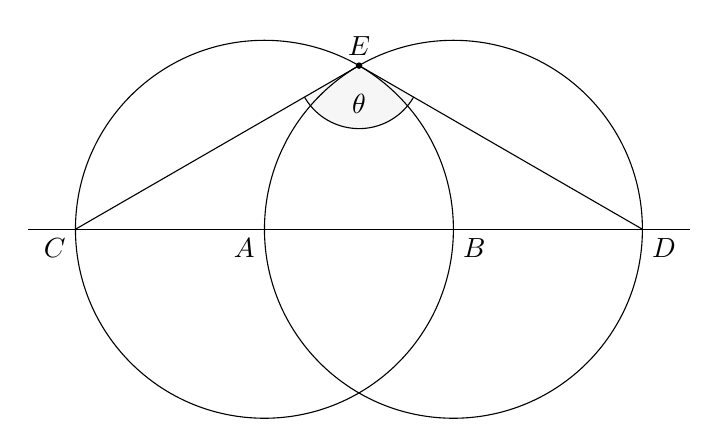
\begin{tikzpicture}
  
    \pic {myfig};

    \begin{pgfonlayer}{bg}% background layer
      \pic [draw=black, fill=gray!7, angle radius=0.8cm,"$\theta$"] at (0,0) {angle = C--intersection-1--D};
    \end{pgfonlayer}

  \end{tikzpicture}
\end{standalonepage}


\begin{standalonepage}
  \begin{tikzpicture}[scale=\scale]% must match scope in myfig
  
    \pic (original) {myfig};
    
    % mark radii
    \draw [green!50!black,thick] (A) -- (B) node[midway,below] {$r$};
    \draw [green!50!black,thick] (A) -- (intersection-1) node[midway,left] {$r$};
    \draw [green!50!black,thick] (intersection-1) -- (B) node[midway,right] {$r$};
    \draw [green!50!black,thick] (A) -- (C) node[midway,below] {$r$};
        
  \end{tikzpicture}
\end{standalonepage}




\begin{standalonepage}
  \begin{tikzpicture}[scale=\scale]% must match scope in myfig
  
    \pic (original) {myfig};
  
    \draw [blue, thick] (A) -- (intersection-1) -- (B) -- cycle;
    
    \pic [draw=blue, text=blue, angle radius=20pt, below, "$60^{\circ}$"{yshift=4pt}, font=\scriptsize]%
      {angle=A--intersection-1--B};
  
    \pic [draw=blue, text=blue, angle radius=20pt, "$60^{\circ}$", font=\scriptsize]%
      {angle=intersection-1--B--A};
    
    \pic [draw=blue, text=blue, angle radius=20pt, "$60^{\circ}$", font=\scriptsize]%
      {angle=B--A--intersection-1};
    
  \end{tikzpicture}
\end{standalonepage}


\begin{standalonepage}
  \begin{tikzpicture}[scale=\scale]% must match scope in myfig
  
    \pic (original) {myfig};
  
    \draw [red, thick] (intersection-1) -- (A) -- (C);
      
    \pic [draw=blue, text=blue, angle radius=20pt, "$60^{\circ}$", font=\scriptsize] {angle=B--A--intersection-1};
    
    \pic [draw=red, triple arc, text=red, angle radius=20pt, "$120^{\circ}$"{xshift={-1pt},yshift={-3pt}}, font=\scriptsize] {angle=intersection-1--A--C};
    
    \pic [draw=red, double arc, text=red, angle radius=30pt, "$30^{\circ}$"{xshift={3pt},yshift={0pt}}, font=\scriptsize] {angle=A--C--intersection-1};
  
    \pic [draw=red, double arc, text=red, angle radius=30pt, "$30^{\circ}$"{xshift={-3pt},yshift={-3pt}}, font=\scriptsize] {angle=C--intersection-1--A};
 

  \end{tikzpicture}
\end{standalonepage}



\begin{standalonepage}
  \begin{tikzpicture}[scale=\scale]% must match scope in myfig
  
    \pic (original) {myfig};
  
    \draw [black] (A) -- (intersection-1) -- (B);

    \pic [draw=blue, text=blue, angle radius=25pt, below, "$60^{\circ}$"{yshift=4pt}, font=\tiny]%
      {angle=A--intersection-1--B};
    
    \pic [draw=blue, double arc, text=blue, angle radius=35pt, "$30^{\circ}$"{xshift={-1pt},yshift={-5pt}}, font=\tiny] {angle=C--intersection-1--A};
  
    \pic [draw=blue, double arc, text=blue, angle radius=35pt, "$30^{\circ}$"{xshift={5pt},yshift={-5pt}}, font=\tiny] {angle=B--intersection-1--D};

  \end{tikzpicture}
\end{standalonepage}

\end{document}
